% Chapter Template

\chapter{Introduction} % Main chapter title

\label{Chapter1} % Change X to a consecutive number; for referencing this chapter elsewhere, use \ref{ChapterX}

Nowadays we are standing in the time, when the fourth round of the industrial revolutions starts. Each of these revolutions was caused by the technological improvements. First one was caused by change from labor work to the mechanization. The second one was started by electrification, in this revolution electric machines were used instead of the steam based motors. The third revolution was the last one, and it was caused by the digitization and the invention of the logical circuits. When we realize how much did the computers evolved it's logical that also industry has to undergo another revolution.
The upcoming revolution is caused by introducting Internet of Things into industry. \cite{brettel2014virtualization}

\section{Reconfiguration}

Today in the time of fast changes on global market and decreasing lifetime of the product, industry is forced into the philosophical shift. 
Manufacturing has to be quickly moved from mass the production to the mass customization. 
In order to rise to the challenge of these trends, the new operation methods are necessary. Production facilities need to be flexible, adaptable and allow fast changes at little cost.
Flexible production systems nowadays come with the higher cost, because these plants has higher initial cost, but even mor important are the costs of down-times needed to reconfigure such plant. 
Reconfiguration without the need to stop production is necessary. 
This requires the reconfiguration of manufacturing plants on all levels, even the physical reconfiuration. Whatever the solution, it must be simple, flexible, and have limited space requirements. For example one of the simpliest approaches, changing the parameters of software components leads to large program that must count with any possible change combination in advance. 

The physical changes in production resources mean a need for dynamic reconfiguration at the control level. 
In order to achieve the real-time reconfiguration of the manufacturin system, we need new software architectures and support from the execution environment. 

On the figure below, the change needed to be done in the industry is shown. In the current approach control system is divided into layers which are horizontally configurable and the connection of the layers is declared in a static way. Reconfiguration of this kind of control system requires the rebuildinf of the whole pyramide from the bottom. While the new approach with also verticaly and horizontaly configurable. 

\begin{figure}[hbp]
\centering
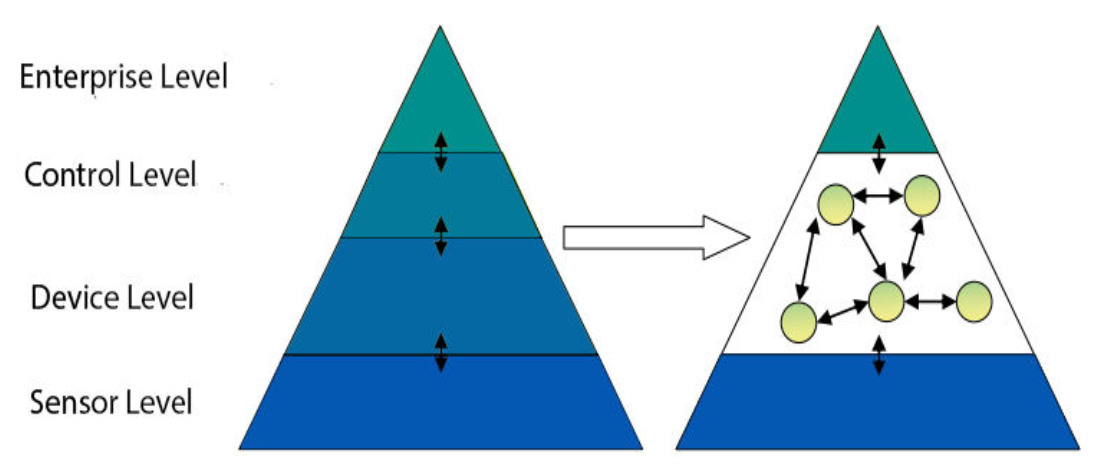
\includegraphics[scale=0.5]{Figures/reconfigurationpyramide}
\decoRule
\caption[Change of industrial pyramide]{sfasdfasdf}
\label{4DIAC IDE System Perspective}
\end{figure}

%----------------------------------------------------------------------------------------
%	Aim of thesis
%----------------------------------------------------------------------------------------

\section{The aim of thesis}
The aim of this thesis is to integrate OPC UA communication protocol into the system 4DIAC - controlling framework based on IEC 61499 standard. 

Controll system created in 4DIAC framework is composed by the function blocks, my task is to implement communication stack inside of function blocks. Including client and also server. 

OPC UA protocol allows user to create topologically ordered web of data. My work also aims to create data topology on the server based on a structure of the control system based on a 4DIAC framework. By the integration of these two technologies, I want to create a system in which all elements of distributed control system could load structure and status of every other element using OPC UA protocol. 



%----------------------------------------------------------------------------------------
%	Chapters overview
%----------------------------------------------------------------------------------------

\section{Chapters overview}
Aim of the following second chapter is to introduce you a IEC 61499 standard and 4DIAC framework based on this standard.
Basic principles of this framework as creating application, function blocks, deploying applications is described.
Important part of using 4DIAC framework is the compiling of your own version of 4DIAC runtime environment dedicated for your device. The whole appendix is dedicated to this topic.

The third chapter is dedicated to communication protocol OPC UA, ways of using this protovol and its information model. I am going to mention stacks based on OPC UA protocol. I am focusing on OPEN 62541 stack, which i have chosen to use in this thesis. 

In the fourth chapter I am explaining my solution of the problem explained in the previous sections of this chapter. Also I am describing the example application to work with OPC UA in 4DIAC.




